
\addtocounter{chapter}{3}
\chapter{Natural Deduction for ML}

\setcounter{ProbPart}{0}

\problempart
Provide proofs for all of the following:
\begin{earg}
\item $\Box (A\eand B)\vdash_K\Box A \eand \Box B$

\myanswer{
\[\begin{nd}
\hypo{1}{\Box (A \eand B)}
\open
\hypo{2}{\hspace{50pt}}
\open
\hypo{3}{A \eand B}
\have{4}{A}\by{$\eand$E}{3}
\close
\have{5}{(A\eand B)\eif A}\by{$\eif$I}{3-4}
\close
\have{6}{\Box((A\eand B)\eif A)}\by{Nec}{2-5}
\have{7}{\Box(A\eand B)\eif \Box A}\by{Dist}{6}
\have{8}{\Box A}\by{$\eif$E}{7,1}
\open
\hypo{9}{\hspace{50pt}}
\open
\hypo{10}{A\eand B}
\have{11}{B}\by{$\eand$E}{10}
\close
\have{12}{(A\eand B)\eif B}\by{$\eif$I}{10-11}
\close
\have{13}{\Box((A\eand B)\eif B)}\by{Nec}{9-12}
\have{14}{\Box(A\eand B)\eif \Box B}\by{Dist}{13}
\have{15}{\Box B}\by{$\eif$E}{14,1}
\have{16}{\Box A \eand \Box B}\by{$\eand$I}{8,15}
\end{nd}\]
}

\item $\Box A\eand\Box B\vdash_K\Box( A \eand  B)$

\myanswer{
\[\begin{nd}
\hypo{1}{\Box A \eand \Box B}
\have{2}{\Box A}\by{$\eand$E}{1}
\have{3}{\Box B}\by{$\eand$E}{2}
\open
\hypo{4}{\hspace{50pt}}
\open
\hypo{5}{A}
\open
\hypo{6}{B}
\have{7}{A\eand B}\by{$\eand$I}{5,6}
\close
\have{8}{B\eif (A\eand B)}\by{$\eif$I}{6-7}
\close
\have{9}{A\eif (B\eif (A\eand B))}\by{$\eif$I}{5-8}
\close
\have{10}{\Box(A \eif (B\eif (A\eand B)))}\by{Nec}{4-9}
\have{11}{\Box A \eif \Box (B\eif (A\eand B))}\by{Dist}{10}
\have{12}{\Box (B\eif (A\eand B))}\by{$\eif$E}{11,2}
\have{13}{\Box B \eif \Box (A\eand B)}\by{Dist}{12}
\have{14}{\Box (A\eand B)}\by{$\eif$E}{13,3}
\end{nd}\]
}

\item $\Box A\eor\Box B\vdash_K\Box( A \eor  B)$

\myanswer{
\[\begin{nd}
\hypo{1}{\Box A \eor \Box B}
\open
\hypo{2}{\Box A}
\open
\hypo{3}{\hspace{50pt}}
\open
\hypo{4}{A}
\have{5}{A\eor B}\by{$\eor$I}{4}
\close
\have{6}{A\eif (A\eor B)}\by{$\eif$I}{4-5}
\close
\have{7}{\Box (A\eif (A\eor B))}\by{Nec}{3-6}
\have{8}{\Box A \eif \Box (A\eor B)}\by{Dist}{7}
\have{9}{\Box(A\eor B)}\by{$\eif$E}{8,2}
\close
\open
\hypo{10}{\Box B}
\open
\hypo{11}{\hspace{50pt}}
\open
\hypo{12}{B}
\have{13}{A\eor B}\by{$\eor$I}{12}
\close
\have{14}{B\eif (A\eor B)}\by{$\eif$I}{12-13}
\close
\have{15}{\Box(B\eif (A\eor B))}\by{Nec}{11-14}
\have{16}{\Box B\eif \Box (A\eor B)}\by{Dist}{15}
\have{17}{\Box (A\eor B)}\by{$\eif$E}{16,10}
\close
\have{18}{\Box(A\eor B)}\by{$\eor$E}{1,2-9,10-17}
\end{nd}\]
}

\item $\Box (A \eiff B)\vdash_K \Box A \eiff \Box B$
\myanswer{
\[\begin{nd}
\hypo{1}{\Box(A\eiff B)}
\open
\hypo{2}{\Box A}
\open
\hypo{3}{\hspace{50pt}}
\open
\hypo{4}{A\eiff B}
\open
\hypo{5}{A}
\have{6}{B}\by{$\eiff$E}{4,5}
\close
\have{7}{A \eif B}\by{$\eif$I}{5-6}
\close
\have{8}{(A\eiff B)\eif (A\eif B)}\by{$\eif$I}{4-7}
\close
\have{9}{\Box((A\eiff B)\eif (A\eif B))}\by{Nec}{3-8}
\have{10}{\Box (A\eiff B)\eif \Box (A\eif B)}\by{Dist}{9}
\have{11}{\Box(A\eif B)}\by{$\eif$E}{10,1}
\have{12}{\Box A \eif \Box B}\by{Dist}{11}
\have{13}{\Box B}\by{$\eif$E}{12,2}
\close
\open
\hypo{14}{\Box B}
\open
\hypo{15}{\hspace{50pt}}
\open
\hypo{16}{A\eiff B}
\open
\hypo{17}{B}
\have{18}{A}\by{$\eiff$E}{16,17}
\close
\have{19}{B\eif A}\by{$\eif$E}{17-18}
\close
\have{20}{(A\eiff B)\eif(B\eif A)}\by{$\eif$E}{16-19}
\close
\have{21}{\Box((A\eiff B)\eif (B\eif A))}\by{Nec}{15-20}
\have{22}{\Box(A\eiff B)\eif \Box (B\eif A)}\by{Dist}{21}
\have{23}{\Box(B\eif A)}\by{$\eif$E}{22,1}
\have{24}{\Box B \eif \Box A}\by{Dist}{23}
\have{25}{\Box A}\by{$\eif$E}{24,14}
\close
\have{26}{\Box A \eiff \Box B}\by{$\eiff$I}{2-13, 14-25}
\end{nd}\]
}
\end{earg}

\problempart
Provide proofs for the following (without using Modal Conversion!):
\begin{earg}
\item $\enot\Box A\vdash_K \Diamond \enot A$
\myanswer{
\[\begin{nd}
\hypo{1}{\enot\Box A}
\open
\hypo{2}{\hspace{50pt}}
\open
\hypo{3}{\enot\enot A}
\have{4}{A}\by{DNE}{3}
\close
\have{5}{\enot\enot A\eif A}\by{$\eif$I}{3-4}
\close
\have{6}{\Box(\enot \enot A\eif A)}\by{Nec}{3-5}
\have{7}{\Box\enot\enot A\eif \Box A}\by{Dist}{6}
\have{8}{\enot\Box\enot\enot A}\by{MT}{7,1}
\have{9}{\Diamond\enot A}\by{$\Diamond$Def}{8}
\end{nd}\]
}

\item $\Diamond\enot A\vdash_K\enot \Box A$
\myanswer{
\[\begin{nd}
\hypo{1}{\Diamond\enot A}
\have{2}{\enot\Box\enot \enot A}\by{$\Diamond$Def}{1}
\open
\hypo{3}{\hspace{50pt}}
\open
\hypo{4}{A}
\open
\hypo{5}{\enot A}
\have{6}{\bot}\by{$\bot$I}{4,5}
\close
\have{7}{\enot\enot A}\by{$\enot$I}{5-6}
\close
\have{8}{A\eif \enot\enot A}\by{$\eif$I}{5-7}
\close
\have{9}{\Box(A\eif \enot \enot A)}\by{Nec}{3-8}
\have{10}{\Box A\eif \Box\enot\enot A}\by{Dist}{9}
\have{11}{\enot\Box A}\by{MT}{10,2}
\end{nd}\]
}

\item $\enot\Diamond A\vdash_K\Box\enot A$

\myanswer{
\[\begin{nd}
\hypo{1}{\enot\Diamond A}
\open
\hypo{2}{\enot\Box\enot A}
\have{3}{\Diamond A}\by{$\Diamond$Def}{2}
\have{4}{\bot}\by{$\bot$I}{3,1}
\close
\have{5}{\enot\enot\Box\enot A}\by{$\enot$I}{2-4}
\have{6}{\Box \enot A}\by{DNE}{5}
\end{nd}\]
}

\item $\Box\enot A\vdash_K\enot\Diamond A$
\myanswer{
\[\begin{nd}
\hypo{1}{\Box\enot A}
\open
\hypo{2}{\Diamond A}
\have{3}{\enot \Box \enot A}\by{$\Diamond$Def}{2}
\have{4}{\bot}\by{$\bot$I}{1,3}
\close
\have{5}{\enot\Diamond A}\by{$\enot$I}{2-4}
\end{nd}\]
}
\end{earg}

\problempart
Provide proofs of the following (and now feel free to use Modal Conversion!):
\begin{earg}
\item $\Box(A\eif B), \Diamond A \vdash_K \Diamond B$
\myanswer{
\[\begin{nd}
\have{1}{\Box(A\eif B)}
\hypo{2}{\Diamond A}
\have{3}{\enot\Box\enot A}\by{$\Diamond$Def}{2}
\open
\hypo{4}{\hspace{50pt}}
\open
\hypo{5}{A\eif B}
\open
\hypo{6}{\enot B}
\have{7}{\enot A}\by{MT}{5,6}
\close
\have{8}{\enot B\eif \enot A}\by{$\eif$I}{6-7}
\close
\have{9}{(A\eif B)\eif (\enot B\eif \enot A)}\by{$\eif$I}{5-8}
\close
\have{10}{\Box((A\eif B)\eif (\enot B\eif \enot A))}\by{Nec}{4-9}
\have{11}{\Box(A\eif B)\eif \Box (\enot B\eif \enot A)}\by{Dist}{10}
\have{12}{\Box(\enot B\eif \enot A)}\by{$\eif$E}{11,1}
\have{13}{\Box\enot B\eif \Box\enot A}\by{Dist}{12}
\have{14}{\enot\Box\enot B}\by{MT}{13,3}
\have{15}{\Diamond B}\by{$\Diamond$Def}{14}
\end{nd}\]
}

\item $\Box A \vdash_K \enot\Diamond\enot A$
\myanswer{
\[\begin{nd}
\hypo{1}{\Box A}
\open
\hypo{2}{\enot\enot\Diamond\enot A}
\have{3}{\Diamond\enot A}\by{DNE}{2}
\have{4}{\enot\Box A}\by{MC}{3}
\have{5}{\bot}\by{$\bot$I}{1,4}
\close
\have{6}{\enot\enot\enot\Diamond\enot A}\by{$\enot$I}{2-5}
\have{7}{\enot\Diamond\enot A}\by{DNE}{6}
\end{nd}\]
}

\item $\enot\Diamond\enot A \vdash_K \Box A$
\myanswer{
\[\begin{nd}
\hypo{1}{\enot\Diamond\enot A}
\have{2}{\Box\enot\enot A}\by{MC}{1}
\open
\hypo{3}{\hspace{50pt}}
\open
\hypo{4}{\enot\enot A}
\have{5}{A}\by{DNE}{4}
\close
\have{6}{\enot\enot A\eif A}\by{$\eif$I}{4-5}
\close
\have{7}{\Box(\enot\enot A \eif A)}\by{Nec}{3-6}
\have{8}{\Box\enot\enot A\eif \Box A}\by{Dist}{7}
\have{9}{\Box A}\by{$\eif$E}{7,2}
\end{nd}\]
}
\end{earg}

\problempart
Provide proofs for the following:
\begin{earg}
\item $P\vdash_T\Diamond P$
\myanswer{
\[\begin{nd}
\hypo{1}{P}
\open
\hypo{3}{\Box \enot P}
\have{4}{\enot P}\by{$T$}{3}
\have{5}{\bot}\by{$\bot$I}{1,4}
\close
\have{6}{\enot\Box\enot P}\by{$\enot$I}{3-5}
\have{7}{\Diamond P}\by{$\Diamond$Def}{6}
\end{nd}\]
}

\item $\vdash_T (A\eand B)\eor(\enot \Box A\eor\enot\Box B)$
\myanswer{
\[\begin{nd}
\open
\hypo{1}{\Box A\eand\Box B}
\have{2}{\Box A}\by{$\eand$E}{1}
\have{3}{\Box B}\by{$\eand$E}{1}
\have{4}{A}\by{$T$}{2}
\have{5}{B}\by{$T$}{3}
\have{6}{A\eand B}\by{$\eand$I}{4,5}
\have{7}{(A\eand B)\eor (\enot \Box A\eor \enot \Box B)}\by{$\eor$I}{6}
\close
\open
\hypo{8}{\enot(\Box A\eand \Box B)}
\have{9}{\enot\Box A \eor \enot\Box B}\by{DeM}{8}
\have{10}{(A\eand B)\eor (\enot\Box A \eor \enot\Box B)}\by{$\eor$I}{9}
\close
\have{11}{(A\eand B)\eor (\enot\Box A \eor \enot\Box B)}\by{TND}{1-7,8-10}
\end{nd}\]
}
\end{earg}

\problempart
Provide proofs for the following:
\begin{earg}
\item $\Box(\Box A\eif B), \Box (\Box B\eif C), \Box A \vdash_{S4}\Box\Box B \eand \Box\Box\Box C$

\myanswer{
\[\begin{nd}
\have{1}{\Box(\Box A \eif B)}
\have{2}{\Box(\Box B\eif C)}
\hypo{3}{\Box A}
\have{4}{\Box \Box A}\by{$S4$}{3}
\have{5}{\Box\Box A\eif \Box B}\by{Dist}{1}
\have{6}{\Box B}\by{$\eif$E}{5,4}
\have{7}{\Box \Box B}\by{$S4$}{6}
\have{8}{\Box \Box B\eif \Box C}\by{Dist}{2}
\have{9}{\Box C}\by{$\eif$E}{8,7}
\have{10}{\Box \Box C}\by{$S4$}{9}
\have{11}{\Box\Box\Box C}\by{$S4$}{10}
\have{12}{\Box\Box B \eand \Box\Box\Box C}\by{$\eand$I}{7,11}
\end{nd}\]
}

\item $\Box A \vdash_{S4} \Box(\Box A \eor B)$
\myanswer{
\[\begin{nd}
\hypo{1}{\Box A}
\have{2}{\Box\Box A}\by{$S4$}{1}
\open
\hypo{3}{\hspace{50pt}}
\open
\hypo{4}{\Box A}
\have{5}{\Box A \eor B}\by{$\eor$I}{4}
\close
\have{6}{\Box A\eif (\Box A \eor B)}\by{$\eif$I}{4-5}
\close
\have{7}{\Box(\Box A \eif (\Box A \eor B))}\by{Nec}{3-6}
\have{8}{\Box\Box A \eif \Box(\Box A \eor B)}\by{Dist}{7}
\have{9}{\Box(\Box A \eor B)}\by{$\eif$E}{8,2}
\end{nd}\]
}

\item $\Diamond \Diamond A \vdash_{S4} \Diamond A$
\myanswer{
\[\begin{nd}
\hypo{1}{\Diamond\Diamond A}
\open
\hypo{2}{\enot\Diamond A}
\have{3}{\Box \enot A}\by{MC}{2}
\have{4}{\Box\Box\enot A}\by{$S4$}{3}
\open
\hypo{5}{\hspace{50pt}}
\open
\hypo{6}{\Box\enot A}
\have{7}{\enot\Diamond A}\by{MC}{6}
\close
\have{8}{\Box\enot A \eif \enot\Diamond A}\by{$\eif$I}{6-7}
\close
\have{9}{\Box(\Box\enot A \eif \enot \Diamond A)}\by{Nec}{5-8}
\have{10}{\Box\Box\enot A \eif \Box\enot\Diamond A}\by{Dist}{9}
\have{11}{\Box\enot\Diamond A}\by{$\eif$E}{10,4}
\have{12}{\enot\Diamond\Diamond A}\by{MC}{11}
\have{13}{\bot}\by{$\bot$I}{1,12}
\close
\have{14}{\enot\enot\Diamond A}\by{$\enot$I}{2-13}
\have{15}{\Diamond A}\by{DNE}{14}
\end{nd}\]
}
\end{earg}

\problempart
Provide proofs for the following:
\begin{earg}
\item $\enot\Box\enot A, \Diamond B\vdash_{S5}\Box(\Diamond A \eand \Diamond B)$
\myanswer{
\[\begin{nd}
\have{1}{\enot\Box\enot A}
\hypo{2}{\Diamond B}
\have{3}{\Diamond A}\by{$\Diamond$Def}{1}
\have{4}{\Box\Diamond A}\by{$S5$}{3}
\have{5}{\Box\Diamond B}\by{$S5$}{2}
\open
\hypo{7}{\hspace{50pt}}
\open
\hypo{8}{\Diamond A}
\open
\hypo{9}{\Diamond B}
\have{10}{\Diamond A \eand \Diamond B}\by{$\eand$I}{8,9}
\close
\have{11}{\Diamond B\eif (\Diamond A \eand \Diamond B)}\by{$\eif$I}{9-10}
\close
\have{12}{\Diamond A\eif (\Diamond B\eif (\Diamond A \eand \Diamond B))}\by{$\eif$I}{8-11}
\close
\have{13}{\Box(\Diamond A\eif (\Diamond B\eif (\Diamond A \eand \Diamond B)))}\by{Nec}{7-12}
\have{14}{\Box\Diamond A \eif \Box (\Diamond B\eif (\Diamond A \eand \Diamond B))}\by{Dist}{13}
\have{15}{\Box(\Diamond B\eif (\Diamond A \eand\Diamond B))}\by{$\eif$E}{14,4}
\have{16}{\Box\Diamond B\eif \Box(\Diamond A \eand \Diamond B)}\by{Dist}{15}
\have{17}{\Box(\Diamond A \eand \Diamond B)}\by{$\eif$E}{16,5}
\end{nd}\]
}

\item $\Diamond\Box A\vdash_{S5}\Box A$
\myanswer{
\[\begin{nd}
\hypo{1}{\Diamond\Box A}
\open
\hypo{2}{\enot\Box A}
\have{3}{\Diamond \enot A}\by{MC}{2}
\have{4}{\Box\Diamond\enot A}\by{$S5$}{3}
\open
\hypo{5}{\hspace{50pt}}
\open
\hypo{6}{\Diamond \enot A}
\have{7}{\enot \Box A}\by{MC}{6}
\close
\have{8}{\Diamond\enot A \eif \enot \Box A}\by{$\eif$I}{6-7}
\close
\have{9}{\Box(\Diamond\enot A \eif \enot\Box A)}\by{Nec}{5-8}
\have{10}{\Box\Diamond\enot A\eif\Box\enot\Box A}\by{Dist}{9}
\have{11}{\Box\enot\Box A}\by{$\eif$E}{10,4}
\have{12}{\enot\Diamond\Box A}\by{MC}{11}
\have{13}{\bot}\by{$\bot$I}{12,1}
\close
\have{14}{\enot\enot\Box A}\by{$\enot$I}{2-13}
\have{15}{\Box A}\by{DNE}{14}
\end{nd}\]
}

\item $\Box A\vdash_{S5}\Box\Box A$
\myanswer{
\[\begin{nd}
\hypo{1}{\Box A}
\open
\hypo{2}{\enot \Diamond \Box A}
\have{3}{\Box\enot\Box A}\by{MC}{2}
\have{4}{\enot\Box A}\by{$T$}{3}
\have{5}{\bot}\by{$\bot$I}{1,4}
\close
\have{6}{\enot\enot\Diamond\Box A}\by{$\enot$I}{2-5}
\have{7}{\Diamond\Box A}\by{DNE}{6}
\have{8}{\Box\Diamond\Box A}\by{$S5$}{7}
\open
\hypo{9}{\hspace{50pt}}
\open
\hypo{10}{\Diamond\Box A}
\open
\hypo{11}{\enot\Box A}
\have{12}{\Diamond\enot A}\by{MC}{11}
\have{13}{\Box\Diamond\enot A}\by{$S5$}{12}
\open
\hypo{14}{\hspace{50pt}}
\open
\hypo{15}{\Diamond \enot A}
\have{16}{\enot\Box A}\by{MC}{15}
\close
\have{17}{\Diamond \enot A\eif \enot \Box A}\by{$\eif$I}{15-16}
\close
\have{18}{\Box(\Diamond\enot A \eif \enot \Box A)}\by{Nec}{14-17}
\have{19}{\Box\Diamond\enot A \eif \Box\enot\Box A}\by{Dist}{18}
\have{20}{\Box\enot\Box A}\by{$\eif$E}{19,13}
\have{21}{\enot\Diamond\Box A}\by{MC}{20}
\have{22}{\bot}\by{$\bot$I}{10,21}
\close
\have{23}{\enot\enot \Box A}\by{$\enot$I}{11-22}
\have{24}{\Box A}\by{DNE}{23}
\close
\have{25}{\Diamond\Box A \eif \Box A}\by{$\eif$I}{10-24}
\close
\have{26}{\Box(\Diamond\Box A \eif \Box A)}\by{Nec}{9-25}
\have{27}{\Box\Diamond\Box A \eif \Box \Box A}\by{Dist}{26}
\have{28}{\Box\Box A}\by{$\eif$E}{27,8}
\end{nd}\]
}
\end{earg}

\chapter{Semantics for ML}

We have presented all of the counter-interpretations diagrammatically. If you would prefer to write them out explicitly, then that would be fine too!

\setcounter{ProbPart}{0}

\problempart
Present counter-interpretations to the following:
\begin{earg}
\item $\enot P \vDash_K \enot\Diamond P$
\myanswer{
\begin{center}
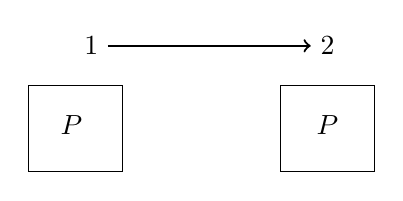
\begin{tikzpicture}
\node (atom1) at (0,1) {1};
\node (atom2) at (3,1) {2};
\node (atom3) at (-0.25,0) {$\enot P$};
\node (atom4) at (3,0) {$P$};
\draw[->, thick] (atom1) -- (atom2);
\draw (-0.8,-0.6) rectangle (0.4,0.5);
\draw (2.4,-0.6) rectangle (3.6,0.5);
\end{tikzpicture}
\end{center}
}

\item $\Box(P \eor Q)\vDash_K \Box P \eor \Box Q$
\myanswer{
\begin{center}
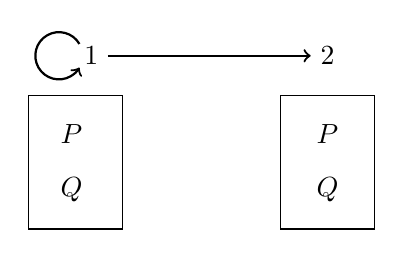
\begin{tikzpicture}
\node (atom1) at (0,1) {1};
\node (atom2) at (3,1) {2};
\node (atom3) at (-0.25,0) {$P$};
\node (atom4) at (3,0) {$\enot P$};
\node (atom5) at (-0.25,-0.7) {$\enot Q$};
\node (atom6) at (3,-0.7) {$Q$};
\draw[->, thick] (atom1)+(-0.15,0.15) arc (-330:-30:.3); 
%\draw[->, thick] (atom2)+(0.15,-0.15) arc (-150:150:.3); 
\draw[->, thick] (atom1) -- (atom2);
\draw (-0.8,-1.2) rectangle (0.4,0.5);
\draw (2.4,-1.2) rectangle (3.6,0.5);
\end{tikzpicture}
\end{center}
}

\item $\vDash_K \enot \Box (A\eand \enot A)$
\myanswer{
\begin{center}
\begin{tikzpicture}
\node (atom1) at (0,1) {1};
\node (atom3) at (-0,0) {$\enot A$};
\draw (-0.5,-0.6) rectangle (0.6,0.5);
\end{tikzpicture}
\end{center}
}

\item $\Box A\vDash_K A$
\myanswer{
\begin{center}
\begin{tikzpicture}
\node (atom1) at (0,1) {1};
\node (atom2) at (3,1) {2};
\node (atom3) at (-0.25,0) {$\enot A$};
\node (atom4) at (3,0) {$A$};
\draw[->, thick] (atom1) -- (atom2);
\draw (-0.8,-0.6) rectangle (0.4,0.5);
\draw (2.4,-0.6) rectangle (3.6,0.5);
\end{tikzpicture}
\end{center}
}
\end{earg}

\problempart
Present counter-interpretations to the following:
\begin{earg}
\item $\Box (M\eif O),\Diamond M\vDash_T O$
\myanswer{
\begin{center}
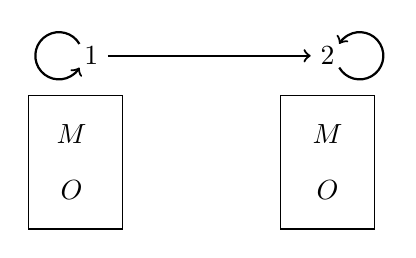
\begin{tikzpicture}
\node (atom1) at (0,1) {1};
\node (atom2) at (3,1) {2};
\node (atom3) at (-0.25,0) {$\enot M$};
\node (atom4) at (3,0) {$M$};
\node (atom5) at (-0.25,-0.7) {$\enot O$};
\node (atom6) at (3,-0.7) {$O$};
\draw[->, thick] (atom1)+(-0.15,0.15) arc (-330:-30:.3); 
%\draw[->, thick] (atom2)+(0.15,-0.15) arc (-150:150:.3); 
\draw[->, thick] (atom1) -- (atom2);
\draw[->, thick] (atom2)+(0.15,-0.15) arc (-150:150:.3); 
\draw (-0.8,-1.2) rectangle (0.4,0.5);
\draw (2.4,-1.2) rectangle (3.6,0.5);
\end{tikzpicture}
\end{center}
}

\item $\Box A\vDash_T \Box \Box A$
\myanswer{
\begin{center}
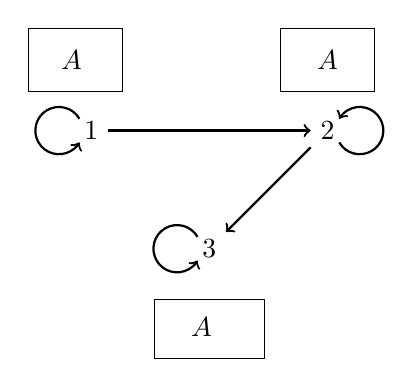
\begin{tikzpicture}
\node (atom1) at (0,1) {1};
\node (atom2) at (3,1) {2};
\node (atom3) at (1.5,-0.5) {3};
\node (atom4) at (-0.25,1.9) {$A$};
\node (atom5) at (3,1.9) {$A$};
\node (atom6) at (1.4,-1.5) {$\enot A$};
\draw[->, thick] (atom1)--(atom2);
\draw[->, thick] (atom1)+(-0.15,0.15) arc (-330:-30:.3); 
\draw[->, thick] (atom2)+(0.15,-0.15) arc (-150:150:.3); 
\draw[->, thick] (atom2)--(atom3);
\draw[->, thick] (atom3)+(-0.15,0.15) arc (-330:-30:.3); 
\draw (-0.8,1.5) rectangle (0.4,2.3);
\draw (2.4,1.5) rectangle (3.6,2.3);
\draw (0.8,-1.15) rectangle (2.2,-1.9);
\end{tikzpicture}
\end{center}
}
\end{earg}

\problempart
Present counter-interpretations to the following:
\begin{earg}
\item $\Diamond A\vDash_{S4} \Box\Diamond A$
\myanswer{
\begin{center}
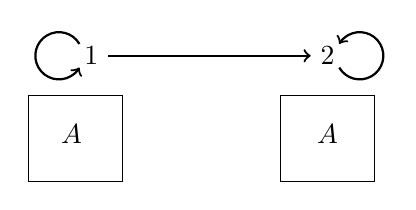
\begin{tikzpicture}
\node (atom1) at (0,1) {1};
\node (atom2) at (3,1) {2};
\node (atom3) at (-0.25,0) {$A$};
\node (atom4) at (3,0) {$\enot A$};
\draw[->, thick] (atom1)+(-0.15,0.15) arc (-330:-30:.3); 
\draw[->, thick] (atom2)+(0.15,-0.15) arc (-150:150:.3); 
\draw[->, thick] (atom1) -- (atom2);
\draw (-0.8,-0.6) rectangle (0.4,0.5);
\draw (2.4,-0.6) rectangle (3.6,0.5);
\end{tikzpicture}
\end{center}
}

\item $\Diamond A, \Box (\Diamond A \eif B)\vDash_{S4}\Box B$

\myanswer{
\begin{center}
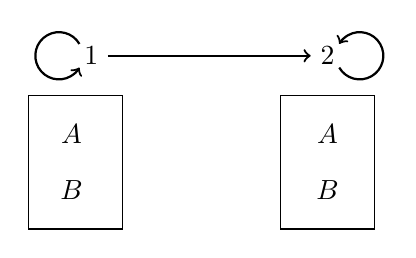
\begin{tikzpicture}
\node (atom1) at (0,1) {1};
\node (atom2) at (3,1) {2};
\node (atom3) at (-0.25,0) {$A$};
\node (atom4) at (3,0) {$\enot A$};
\node (atom5) at (-0.25,-0.7) {$B$};
\node (atom6) at (3,-0.7) {$\enot B$};
\draw[->, thick] (atom1)+(-0.15,0.15) arc (-330:-30:.3); 
\draw[->, thick] (atom2)+(0.15,-0.15) arc (-150:150:.3); 
\draw[->, thick] (atom1) -- (atom2);
\draw (-0.8,-1.2) rectangle (0.4,0.5);
\draw (2.4,-1.2) rectangle (3.6,0.5);
\end{tikzpicture}
\end{center}
}
\end{earg}
